%%%%%%%%%%%%%%%%%%%%%%%%%%%%%%%%%%%%%%%%%
% Structured General Purpose Assignment
% LaTeX Template
%
% This template has been downloaded from:
% http://www.latextemplates.com
%
% Original author:
% Ted Pavlic (http://www.tedpavlic.com)
%
% Note:
% The \lipsum[#] commands throughout this template generate dummy text
% to fill the template out. These commands should all be removed when 
% writing assignment content.
%
%%%%%%%%%%%%%%%%%%%%%%%%%%%%%%%%%%%%%%%%%

%----------------------------------------------------------------------------------------
%	PACKAGES AND OTHER DOCUMENT CONFIGURATIONS
%----------------------------------------------------------------------------------------

\documentclass{article}

\usepackage{fancyhdr} % Required for custom headers
\usepackage{lastpage} % Required to determine the last page for the footer
\usepackage{extramarks} % Required for headers and footers
\usepackage{graphicx} % Required to insert images
\usepackage{lipsum} % Used for inserting dummy 'Lorem ipsum' text into the template
\usepackage{listings}
\usepackage{color}
\usepackage{amsmath}
\usepackage{hyperref}

\definecolor{dkgreen}{rgb}{0,0.6,0}
\definecolor{gray}{rgb}{0.5,0.5,0.5}
\definecolor{mauve}{rgb}{0.58,0,0.82}

\lstset{frame=tb,
  language=c,
  aboveskip=3mm,
  belowskip=3mm,
  showstringspaces=false,
  columns=flexible,
  basicstyle={\small\ttfamily},
  numbers=none,
  numberstyle=\tiny\color{gray},
  keywordstyle=\color{blue},
  commentstyle=\color{dkgreen},
  stringstyle=\color{mauve},
  breaklines=true,
  breakatwhitespace=true
  tabsize=3
}

% Margins
\topmargin=-0.45in
\evensidemargin=0in
\oddsidemargin=0in
\textwidth=6.5in
\textheight=9.0in
\headsep=0.25in 

\linespread{1.1} % Line spacing

% Set up the header and footer
\pagestyle{fancy}
\lhead{\hmwkAuthorName} % Top left header
\chead{\hmwkClass\ (\hmwkClassInstructor\ \hmwkClassTime): \hmwkTitle} % Top center header
\rhead{\firstxmark} % Top right header
\lfoot{\lastxmark} % Bottom left footer
\cfoot{} % Bottom center footer
\rfoot{Page\ \thepage\ of\ \pageref{LastPage}} % Bottom right footer
\renewcommand\headrulewidth{0.4pt} % Size of the header rule
\renewcommand\footrulewidth{0.4pt} % Size of the footer rule

\setlength\parindent{0pt} % Removes all indentation from paragraphs

%----------------------------------------------------------------------------------------
%	DOCUMENT STRUCTURE COMMANDS
%	Skip this unless you know what you're doing
%----------------------------------------------------------------------------------------

% Header and footer for when a page split occurs within a problem environment
\newcommand{\enterProblemHeader}[1]{
\nobreak\extramarks{#1}{#1 continued on next page\ldots}\nobreak
\nobreak\extramarks{#1 (continued)}{#1 continued on next page\ldots}\nobreak
}

% Header and footer for when a page split occurs between problem environments
\newcommand{\exitProblemHeader}[1]{
\nobreak\extramarks{#1 (continued)}{#1 continued on next page\ldots}\nobreak
\nobreak\extramarks{#1}{}\nobreak
}

\setcounter{secnumdepth}{0} % Removes default section numbers
\newcounter{homeworkProblemCounter} % Creates a counter to keep track of the number of problems

\newcommand{\homeworkProblemName}{}
\newenvironment{homeworkProblem}[1][Problem \arabic{homeworkProblemCounter}]{ % Makes a new environment called homeworkProblem which takes 1 argument (custom name) but the default is "Problem #"
\stepcounter{homeworkProblemCounter} % Increase counter for number of problems
\renewcommand{\homeworkProblemName}{#1} % Assign \homeworkProblemName the name of the problem
\section{\homeworkProblemName} % Make a section in the document with the custom problem count
\enterProblemHeader{\homeworkProblemName} % Header and footer within the environment
}{
\exitProblemHeader{\homeworkProblemName} % Header and footer after the environment
}

\newcommand{\problemAnswer}[1]{ % Defines the problem answer command with the content as the only argument
\noindent\framebox[\columnwidth][c]{\begin{minipage}{0.98\columnwidth}#1\end{minipage}} % Makes the box around the problem answer and puts the content inside
}

\newcommand{\homeworkSectionName}{}
\newenvironment{homeworkSection}[1]{ % New environment for sections within homework problems, takes 1 argument - the name of the section
\renewcommand{\homeworkSectionName}{#1} % Assign \homeworkSectionName to the name of the section from the environment argument
\subsection{\homeworkSectionName} % Make a subsection with the custom name of the subsection
\enterProblemHeader{\homeworkProblemName\ [\homeworkSectionName]} % Header and footer within the environment
}{
\enterProblemHeader{\homeworkProblemName} % Header and footer after the environment
}
   
%----------------------------------------------------------------------------------------
%	NAME AND CLASS SECTION
%----------------------------------------------------------------------------------------

\newcommand{\hmwkTitle}{Assignment\ \#7} % Assignment title
\newcommand{\hmwkDueDate}{Monday,\ May 5,\ 2014} % Due date
\newcommand{\hmwkClass}{Computational Biology} % Course/class
\newcommand{\hmwkClassTime}{1:30pm} % Class/lecture time
\newcommand{\hmwkClassInstructor}{Jianyang Zeng} % Teacher/lecturer
\newcommand{\hmwkAuthorName}{Weiyi Chen} % Your name

%----------------------------------------------------------------------------------------
%	TITLE PAGE
%----------------------------------------------------------------------------------------

\title{
\vspace{2in}
\textmd{\textbf{\hmwkClass:\ \hmwkTitle}}\\
\normalsize\vspace{0.1in}\small{Due\ on\ \hmwkDueDate}\\
\vspace{0.1in}\large{\textit{\hmwkClassInstructor\ \hmwkClassTime}}
\vspace{3in}
}

\author{\textbf{\hmwkAuthorName}}
\date{} % Insert date here if you want it to appear below your name

%----------------------------------------------------------------------------------------

\begin{document}

\maketitle

%----------------------------------------------------------------------------------------
%	TABLE OF CONTENTS
%----------------------------------------------------------------------------------------

%\setcounter{tocdepth}{1} % Uncomment this line if you don't want subsections listed in the ToC

%\newpage
%\tableofcontents
\newpage

%----------------------------------------------------------------------------------------
%	PROBLEM 1
%----------------------------------------------------------------------------------------

% To have just one problem per page, simply put a \clearpage after each problem

\begin{homeworkProblem}
	Graph Cut (15 points).
	\begin{homeworkSection}{(1)}
		\centerline{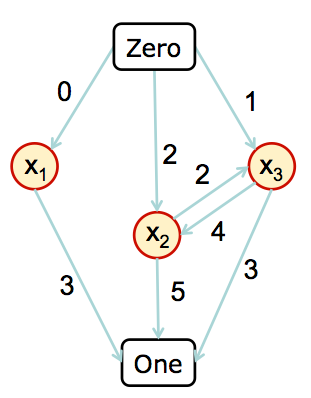
\includegraphics[scale=0.4]{network}}
	\end{homeworkSection}
	\begin{homeworkSection}{(2)}
		The min cut approach, Ford \& Fulkerson algorithm, refers to
		\begin{lstlisting}
Find the path from source to sink
	While (path exists)
		flow += maximum capacity in the path
		Build the residual graph ("subtract" the flow)
		Find the path in the residual graph
	End
		\end{lstlisting}
		\begin{itemize}
			\item Path: $\text{Zero} \rightarrow x_1 \rightarrow \text{One}$, $\text{Flow} = 0$, cut edge $\text{Zero} \rightarrow x_1$
			\item Path: $\text{Zero} \rightarrow x_2 \rightarrow \text{One}$, $\text{Flow} = 2$, cut edge $\text{Zero} \rightarrow x_2$
			\item Path: $\text{Zero} \rightarrow x_3 \rightarrow \text{One}$, $\text{Flow} = 1$, cut edge $\text{Zero} \rightarrow x_3$
 		\end{itemize}
		The resulting graph is as follows. \\
		\centerline{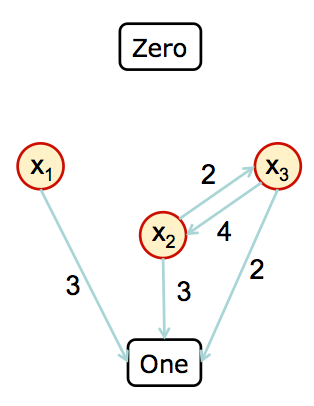
\includegraphics[scale=0.4]{resulting}}
		Therefore, since the cut edges are $\text{Zero} \rightarrow x_1$, $\text{Zero} \rightarrow x_2$ and $\text{Zero} \rightarrow x_3$, then
		$$ x_1 = x_2 = x_3 = 0 $$
		minimizes the energy function as $$E(x) = \phi_1(0) + \phi_2(0) + \phi_{23}(0,0) = 3$$
	\end{homeworkSection}
\end{homeworkProblem}

%----------------------------------------------------------------------------------------
%	PROBLEM 2
%----------------------------------------------------------------------------------------

% To have just one problem per page, simply put a \clearpage after each problem

\begin{homeworkProblem}
	 Belief Propagation (15 points): Let $T$ be a tree factor graph rooted at a variable node $r$. The set of beliefs returned by $BPTree(T)$ are the exact marginal probabilities of the variable nodes of T.
	 \begin{homeworkSection}{Proof}
	 	We divide the proof in two parts. In Part 1, we show by induction on height of the tree and considering messages only from leaves to root, that the belief at the root is exactly the marginal at the root. In Part 2, we prove the correctness of marginals at all other nodes by induction again on height and considering the messages now in the downwards direction, i.e. from root to leaves.
		\begin{itemize}
		\item Notation: Let $H$ be the height of the tree. For $H = 1$, the marginal of the root is trivially equal to the product of its neighboring factors. For a variable node $i$ at height $h$, let $T_{i,h}$ denote the tree rooted at node $i$. We denote the set of variable nodes in $T_{i,h}$ and the set of factor nodes by $A( T_{i,h})$.  Let $X_{T_i}$ denote a configuration of variables in $I(T_{i,h})$. 
		\item \textbf{Part 1.} Assume that for any variable node $i$ at height $h < H$, the belief of $i$ computed as a product of messages received from its neighbors in $T_{i,h}$ is equal to its true marginal in $T_{i,h}$. Now the belief of node $i$ can be written as
		$$ b_r(x_r) \propto \prod_{a \in N(r)} \sum_{X_a / x_r} f_a(X_a) \prod_{i \in N(a) / r} b_i^a(x_i) $$
		where $b_i^a(x_i)$ is the belief of node $i$ in $T_{i,H-2}$. \\
		\centerline{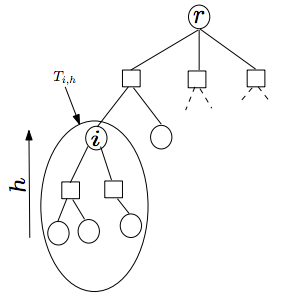
\includegraphics[scale=0.5]{part1}}
		Recall that a variable node $i$ in a factor graph is associated with a random variable $X_i$, which can take a value from its state space $X_i$. A belief of a variable node i, denoted by $b_i(x_i)$ represents the likeness of random variable $X_i$ to take value $x_i \in X_i$. $N(a)$ denotes the neighbors of node $a$ and $f_a(X_a)$ is the function corresponding to the factor node $a$. $b_j^a(x_j)$ is the belief of variable $j$ in a factor graph in which the factor a is removed. Let $P^a_i(x_i)$ be the marginal for node i in $T_{i,H-2}$. By applying the inductive hypothesis, we have
		\begin{align*}
			b_r(x_r) &\propto \prod_{a \in N(r)} \sum_{X_a / x_r} f_a(X_a) \prod_{i \in N(a) / r} P_i^a(x_i) \\
			&\propto \prod_{a \in N(r)} \sum_{X_a / x_r} f_a(X_a) \prod_{i \in N(a) / r} \sum_{X_{T_i}/x_i} \prod_{b \in A(T_{i, H-2})} f_b(X_b) \\
			&\propto \prod_{a \in N(r)} \sum_{X_a / x_r} f_a(X_a)  \sum_{X_{T_i}/x_i, i \in N(a) / r} \prod_i \prod_{b \in A(T_{i, H-2})} f_b(X_b) \\
			&\propto \prod_{a \in N(r)} \sum_{X_a / x_r} \sum_{X_{T_i}/x_i, i \in N(a) / r}  f_a(X_a) \prod_i \prod_{b \in A(T_{i, H-2})} f_b(X_b) \\
			&\propto \sum_{X_a / x_r} \prod_{a \in N(r)} f_a(X_a) \prod_{i \in N(a) / r} \prod_{b \in A(T_{i, H-2})} f_b(X_b) \\
			&\propto \sum_{X_a / x_r} \prod_{a \in N(r)} f_a(X_a)
		\end{align*}
		which is by definition the exact marginal.
		\item \textbf{Part 2.} Now the messages stabilize and do not change for the upward direction. When the root has received correct messages from all of its neighbors, it can compute the outgoing messages. Assume that with the given set of upward and downward messages, the belief of any node $j$ at distance $d \le H - 1$ from the root is the exact marginal in original graph $T$. \\
		\centerline{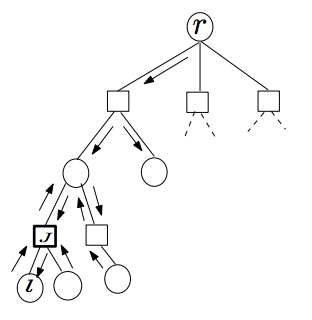
\includegraphics[scale=0.5]{part2}}
		We now prove that, the belief calculated for any leaf is equal to its true marginal in $G$. Indeed, the belief for leaf node $l$ is given by
		\begin{align*}
			b_l(x_l) &\propto \prod_{a \in N(l)} m_{a \rightarrow l} (x_l) \\
			&\propto m_{J \rightarrow l} (x_l) \\
			&\propto \sum_{f_J(X_J)} \sum_{X / X_J} \prod_{b \in A(T) / J} f_b(X_b) \\
			&\propto \sum_{X / x_l} \prod_{b \in A(T)} f_b(X_b)
		\end{align*}
		which is the exact marginal by definition.
		\end{itemize}
	\end{homeworkSection}
\end{homeworkProblem}
\end{document}